\documentclass{VUMIFPSbakalaurinis}
\usepackage{algorithmicx}
\usepackage{algorithm}
\usepackage{algpseudocode}
\usepackage{amsfonts}
\usepackage{amsmath}
\usepackage{bm}
\usepackage{caption}
\usepackage{color}
\usepackage{float}
\usepackage{graphicx}
\usepackage{listings}
\usepackage{subfig}
\usepackage{wrapfig}
\usepackage{makecell}
\usepackage{forest}


\renewcommand\theadfont{\bfseries}

% Titulinio aprašas
\university{Vilniaus universitetas}
\faculty{Matematikos ir informatikos fakultetas}
\department{Programų sistemų katedra}
\papertype{Bakalauro darbas}
\title{Gestų kalbos vienetų atpažinimas iš video srauto}
\titleineng{Recognition of Sign language units from a video stream}
\author{Pranciškus Ambrazas}
\supervisor{j. asist. Linas Petkevičius}
\reviewer{dr. Vytautas Valaitis}
\date{Vilnius – \the\year}

% Nustatymai
% \setmainfont{Palemonas}   % Pakeisti teksto šriftą į Palemonas (turi būti įdiegtas sistemoje)
\bibliography{bibliografija}

\begin{document}
\maketitle

%% Padėkų skyrius
% \sectionnonumnocontent{}
% \vspace{7cm}
% \begin{center}
%     Padėkos asmenims ir/ar organizacijoms
% \end{center}

\sectionnonumnocontent{Santrauka}
Glaustai aprašomas darbo turinys: pristatoma nagrinėta problema ir padarytos
išvados. Santraukos apimtis ne didesnė nei 0,5 puslapio. Santraukų gale
nurodomi darbo raktiniai žodžiai. 
% Nurodomi iki 5 svarbiausių temos raktinių žodžių (terminų).
% Vienas terminas gali susidėti iš kelių žodžių.
\raktiniaizodziai{raktinis žodis 1, raktinis žodis 2, raktinis žodis 3, raktinis žodis 4, raktinis žodis 5}   

\sectionnonumnocontent{Summary}
Santrauka anglų kalba. Santraukos apimtis ne didesnė nei 0,5 puslapio.
\keywords{keyword 1, keyword 2, keyword 3, keyword 4, keyword 5}

\tableofcontents

\sectionnonum{Įvadas}
Pasaulyje yra virš 7 milijardų žmonių, kurie kasdien tarpusavyje komunikuoja. Netgi 5\% visos žmonijos populiacijos sudaro žmonės, turintys klausos problemų. Vien 34 milijonai iš jų yra vaikai, iš kurių net 60\% praradusių klausą vaikystėje galėjo būti girdintys dabar, jei būtų imtąsi atitinkamų prevencinių priemonių. Paskaičiuota, kad iki 2050 metų žmonių, turinčių šias problemas, skaičius išaugs netgi iki 900 milijonų, o vien šiuo metu 1,1 milijardo jaunų žmonių nuo 11 iki 35 metų amžiaus yra ant klausos praradimo ribos dėl per didelio triukšmo \cite{WhoInt}.

\subsectionnonum{Gestų kalba}
Gestų kalba – tai geriausias būdas klausos negalią turintiems žmonėms bendrauti tarpusavyje. Ja pasaulyje bendrauja didžioji dalis klausos sutrikimus turinčiųjų, o amerikiečių gestų kalba (\textit{angl. American Sign Language (ASL)}) yra trečia pagal populiarumą Amerikoje po anglų ir ispanų kalbų, kuria kalba virš 500 tūkstančių žmonių. Kiekviena šalis turi savo valstybinę kalbą - lietuvių, anglų, ispanų, rusų. Lygiai taip pat kiekviena šalis turi ir savo gestų kalbą. Tai yra tiek jau minėta amerikiečių gestų kalba (ASL), lietuvių, argentiniečių ir kitos gestų kalbos. Netgi tam tikri šalių regionai turi specifinius tos pačios kalbos dialektus, kaip, tarkime, vien Lietuvoje yra aukštaičių, žemaičių, suvalkiečių ar dzūkų tarmės. 

Kiekviena gestų kalba turi savo atskirą gramatiką ir sintaksę. Skirtingos gestų kalbos skiriasi tiek abėcėlėmis, tiek pačiais gestais, dėl to skiriasi netgi ta pati gramatika. Taip yra dėl to, kad nėra bendrinės gestų kalbos - vien Amerikoje yra virš 35 skirtingų gestų kalbų. 

Vienas gestas turi turėti kelias prasmes. Kaip ir lietuvių kalboje žodis „kasa“ turi tris skirtingas reikšmes, taip ir gestų kalboje vienas gestas gali turėti keletą reikšmių. Tačiau iš kitos pusės gestas, parodytas truputėlį kitaip gali turėti visiškai priešingą reikšmę. Tarkime, ASL gestai „geras“ ir „blogas“ skiriasi tik puse į kurią atsuktas deltas, tačiau daugiau neturi jokių skirtumų.

\subsectionnonum{Gestų kalbos specifika}
Kiekviena gestų kalba susideda iš \textbf{trijų} pagrindinių dalių:
\begin{enumerate}
	\item\textbf{Statinė gestų kalba} - dar kitaip vadinama \textit{pirštų kalba} (\textit{angl. fingerspelling}). Tai įvairūs gestai rodomi vienos (ASL, LGK) ar net ir dviejų (britų ar vokiečių gestų kalba) rankų pagalba. Tai nejudantys gestai, rodantys vieną raidę (\textit{žr. \ref{img:asl} pav.}) ar net vieną žodį, kaip, pavyzdžiui, ASL „\textit{I love you}“\footnote{liet. Aš tave myliu} gestas. Yra galimybė žodžius išreikšti ir abėcėliškai. Lygiai taip pat žmonės kasdieninėje kalboje turi galimybę pasakyti paraidžiui. Tačiau yra įprasta jungti raides į žodžius. O žodžius galiausiai į sakinius. Vienas iš variantų, kuomet naudojama gestų kalba paraidžiui tai vardų pasakyme. Tačiau gestakalbiai prisistatydami parodo gestą, kuris priklauso tik jiems. Tai tarsi parašas tam, kad nebereikėtų kreipiantis ar apibūdinant žmogų jo vardo sakyti paraidžiui.
	
\begin{figure}[H]
    \centering
    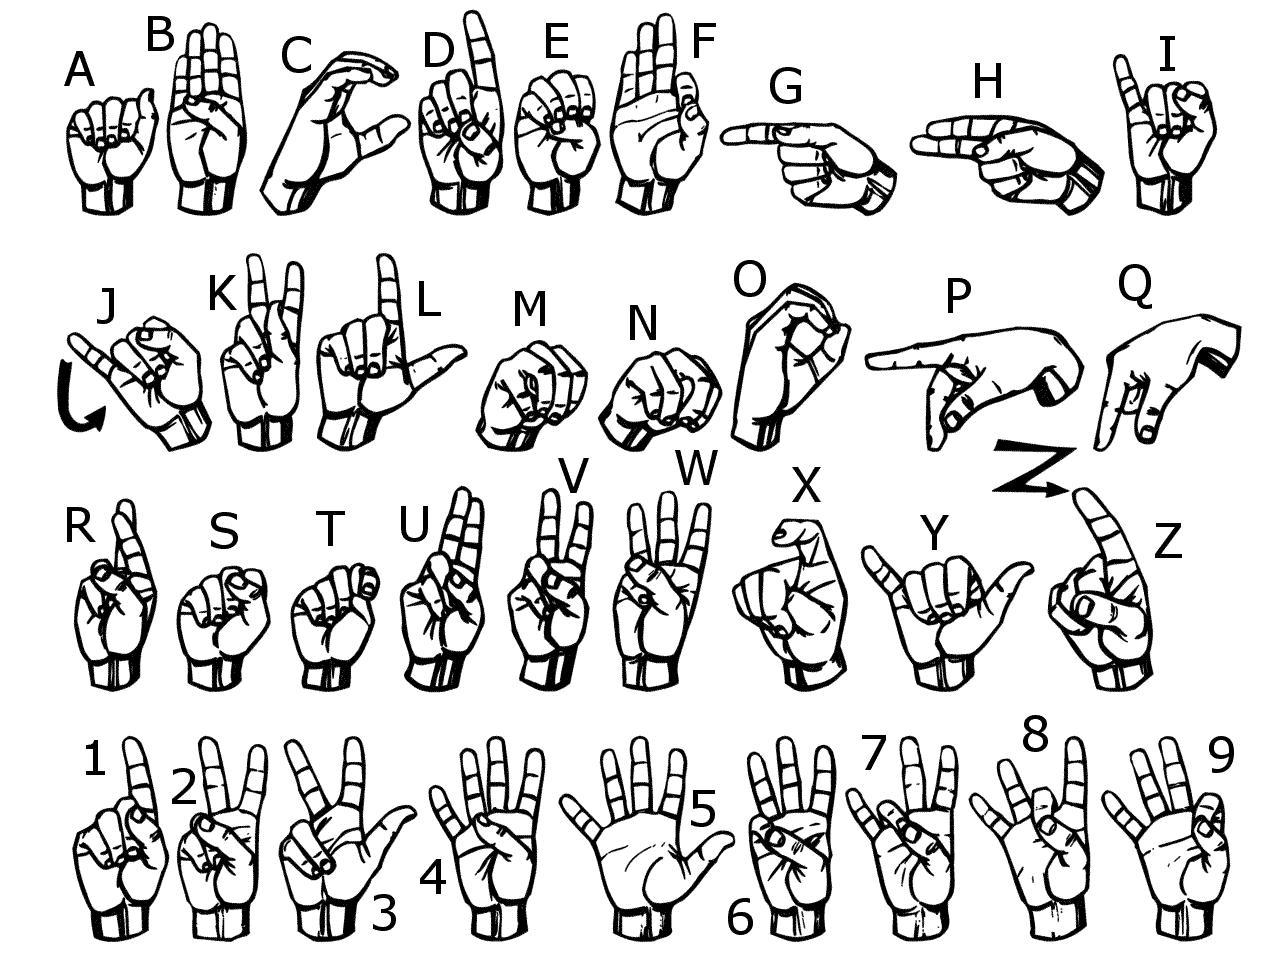
\includegraphics[scale=0.2]{img/ASL}
    \caption{Amerikiečių gestų kalbos abėcėlė}
    \label{img:asl}
\end{figure}

	\item\textbf{Dinaminė gestų kalba} - tai žodžių lygio gestų kalba. Nesunku pastebėti, kad \ref{img:asl} paveikslėlyje yra „J“ ar „Z“ raidės, kurios priskiriama dinaminių judesių klasei. Kaip ir yra žodžių, kurie priskiriami statinei gestų kalbai dėl savo kilmės, taip ir yra raidžių, kurios priskiriamos dinaminei gestų kalbai. Dinaminiais judesiais yra išreiškiami įvairūs gestų kalbos žodžiai tokie, kaip, pavyzdžiui, ASL yra „labas“, „gerai“ ar „blogai“.
	
	\item\textbf{Kitos ypatybės} - emocijos veide, liežuvis, burna ir kūno laikysena. Tai taip pat labai svarbios gestų kalbos ypatybės. Pavyzdžiui, klausiant gestų kalba klausimo, jei bus pakelti antakiai, tai reikš, kad laukiamas ataskymas „taip“ arba „ne“. Tačiau, jei antakiai bus suraukti, tai reikš, kad klausiama su paaiškinimu „kas“, „kur“, „kaip“, „ką“.
\end{enumerate}


\subsectionnonum{Darbo tikslas}
Išanalizuoti gestų kalbos vienetų atpažinimo galimybes ir video srauto.

\subsectionnonum{Darbo uždaviniai}
\begin{itemize}
	\item Gestų kalbos video srautų paieška ir mokomosios medžiagos neuroniniams tinklams surinkimas
	\item Susipažinimas su rekurentiniais neuroniniais tinklais
	\item Gestų kalbos vienetų atpažinimas iš video srauto pasinaudojant rekurentiniais neuroniniais tinklais.
\end{itemize}

\subsectionnonum{Darbo eiga}
\begin{itemize}
	\item Panašių ir jau įgyvendintų projektų paieška
	\item Esamos sistemos patobulinimai
	\item Rezultatų palyginimai
\end{itemize}

\subsectionnonum{Panaudotos priemonės}
\begin{itemize}
	\item Python – programavimo kalba
	\item TensorFlow – skirta darbui su apsimokančiomis sistemomis\footnote{angl. Machine learning}
\end{itemize}



Įvade nurodomas darbo tikslas ir uždaviniai, kuriais bus įgyvendinamas tikslas,
aprašomas temos aktualumas, apibrėžiamas tiriamasis objektas akcentuojant
neapibrėžtumą, kuris bus išspręstas darbe, aptariamos teorinės darbo prielaidos
bei metodika, apibūdinami su tema susiję literatūros ar kitokie šaltiniai,
temos analizės tvarka, darbo atlikimo aplinkybės, pateikiama žinių apie
naudojamus instrumentus (programas ir kt., jei darbe yra eksperimentinė dalis).
Darbo įvadas neturi būti dėstymo santrauka. Įvado apimtis 2–4 puslapiai.


\section{Apsimokančios sistemos}
\textbf{Apsimokančios sistemos} (\textit{angl. machine learning})

\subsection{Prižiūrimas mokymas}
\textbf{Prižiūrimas mokymas} (\textit{angl. supervised learning}) - tai apsimokančių sistemų apmokymo būdas, kuomet duomenys mokymui yra paruošiami taip, kad kiekvienas duomuo turėtų ir atitinkamą rezultatą. Kitaip tariant, jei yra duomuo \textit{a}, tai yra ir jį atitinkantis rezultatas, arba dar vadinama etiketė \textit{b}. Tai būdas, kuris veikia medžio principu.

\begin{table}[H]\footnotesize
  \centering
  \caption{Pavyzdinis prižiūrimo mokymo apmokymui paruoštų duomenų rinkinys}
  {\begin{tabular}{| c | c | c | c | c | c || c |} \hline
    \thead{Nr.} & \thead{Pirštas nr. 1} & \thead{Pirštas nr. 2} & \thead{Pirštas nr. 3} & \thead{Pirštas nr. 4} & \thead{Pirštas nr. 5} & \thead{Raidė} \\
    \hline
    1. & Atlenktas & Užlenktas & Užlenktas & Užlenktas & Užlenktas & \thead{A} \\
    2. & Užlenktas & Atlenktas & Atlenktas & Atlenktas & Atlenktas & \thead{B} \\
    3. & Atlenktas & Sulenktas & Sulenktas & Sulenktas & Sulenktas & \thead{C} \\
    4. & Užlenktas & Atlenktas & Užlenktas & Užlenktas & Užlenktas & \thead{D} \\
    5. & Užlenktas & Užlenktas & Užlenktas & Užlenktas & Užlenktas & \thead{E} \\
    6. & Atlenktas & Užlenktas & Atlenktas & Atlenktas & Atlenktas & \thead{F} \\
    \hline
  \end{tabular}}
  \label{tab:priziurimasPavyzdys}
\end{table}

\ref{tab:priziurimasPavyzdys} lentelėje pateikiamas pavyzdys su amerikiečių gestų kalbos abėcėle. Lentelėje pateikiamos piršų padėtys, o pirštai numeruojami pagal \ref{appendix:pirstai} pateikiamą pirštų numeraciją. Kiekvieno piršto padėtis šiame pavyzdyje gali būti: \textit{atlenktas, sulenktas, užlenktas}. Ir kiekvienai padėčiai esant pateikiamas rezultatas, arba kitaip - etiketė, kokią raidę abėcėlėje atitinka pavaizduotos pirštų padėtys.


\begin{table}[H]\footnotesize
  \centering
  \caption{Pavyzdinė praktinė užduotis}
  {\begin{tabular}{| c | c | c | c | c | c || c |} \hline
    \thead{Nr.} & \thead{Pirštas nr. 1} & \thead{Pirštas nr. 2} & \thead{Pirštas nr. 3} & \thead{Pirštas nr. 4} & \thead{Pirštas nr. 5} & \thead{Raidė} \\
    \hline
    1. & Atlenktas & Sulenktas & Sulenktas & Sulenktas & Sulenktas & \thead{?} \\
    \hline
  \end{tabular}}
  \label{tab:priziurimasUzdavinys}
\end{table}

\ref{tab:priziurimasUzdavinys} lentelėje pateikiamas uždavinys, kuriame nurodoma ta pati informacija, kuri buvo pateikta \ref{tab:priziurimasPavyzdys} lentelėje. Tačiau rezultatas nėra pateiktas, o jis randamas medžio principu.


\begin{figure}[H]
    \centering
    
\begin{forest}
  for tree={
    fit=band,% spaces the tree out a little to avoid collisions
  }
  [\textit{Pirštas nr. 1}
    [Atlenktas
      [\textit{Pirštas nr. 2}
      	[Sulenktas [\textbf{C}]]
	[Užlenktas
	  [\textit{Pirštas nr. 3}
	    [Atlenktas [\textbf{F}]]
	    [Užlenktas [\textbf{A}]]
	  ]
	]
      ]
    ]
    [Užlenktas
      [\textit{Pirštas nr. 2} 
      	[Atlenktas
	  [\textit{Pirštas nr. 3}
	    [Užlenktas [\textbf{D}]]
	    [Atlenktas [\textbf{B}]]
	  ]
	]
      	[Užlenktas [\textbf{E}]]
      ]
    ]  
  ]
\end{forest}
    \caption{Galimybių medis}
    \label{img:medis}
\end{figure}


Vien iš šio medžio galimybių medžio galima matyti, kad pilnai užtenka sprendimui nusakyti 3 pirštų, kadangi rezultatų nėra daug. Jei būtų imama visa abėcėlės aibė, tuomet rezultato nustatymui būtų naudojama galimai visų pirštų padėtys. Tačiau net ir šį medį optimizavus galima būtų, tarkime, C raidė atsakymą gauti tik iš vieno piršto padėties, kadangi tik ši vienintelė raidė turi sulenkto piršto padėtį. Galiausiai iš šio medžio galima pastebėti, kad \ref{tab:priziurimasPavyzdys} lentelėje pateikto pavyzdžio atsakymas yra raidė \textbf{C}.

\subsection{Neprižiūrimas mokymas}
\textbf{Neprižiūrimas mokymas} (\textit{angl. unsupervised learning}) - mokymas, kuomet duomenims nėra priskiriamos teisingos etiketės ar teisingi rezultatai. Pavyzdžiui, tai galėtų atitikti naujos kalbos mokymąsi be mokytojo ir bet kokio žodyno. Kuomet pastoviai matomas vis tas pats tekstas, žodžiai tampa atpažįstami, tačiau išversti jų neišeina. Tačiau tai nesukelia jokių nepatogumų, jei į tekstą reikia įrašyti tinkamą žodį, kuomet dėl daugybės duomenų yra aišku koks žodis su kokia galūne turėtų būti įrašytas.

\begin{table}[H]\footnotesize
  \centering
  \caption{Pavyzdinis neprižiūrimo mokymo apmokymui paruoštų duomenų rinkinys}
  {\begin{tabular}{| c | c | c | c | c | c |} \hline
    \thead{Nr.} & \thead{Pirštas nr. 1} & \thead{Pirštas nr. 2} & \thead{Pirštas nr. 3} & \thead{Pirštas nr. 4} & \thead{Pirštas nr. 5}  \\
    \hline
    1. & Atlenktas & Užlenktas & Užlenktas & Užlenktas & Užlenktas  \\
    2. & Užlenktas & Atlenktas & Atlenktas & Atlenktas & Atlenktas  \\
    3. & Atlenktas & Sulenktas & Sulenktas & Sulenktas & Sulenktas \\
    4. & Užlenktas & Atlenktas & Užlenktas & Užlenktas & Užlenktas \\
    5. & Užlenktas & Užlenktas & Užlenktas & Užlenktas & Užlenktas \\
    6. & Atlenktas & Užlenktas & Atlenktas & Atlenktas & Atlenktas \\
    \hline
  \end{tabular}}
  \label{tab:nepriziurimasPavyzdys}
\end{table}

\ref{tab:nepriziurimasPavyzdys} lentelėje pateikiamas pavyzdinis neprižiūrimam mokymui apmokyti paruoštų duomenų rinkinys. Duomenys tokie patys, kaip ir \ref{tab:priziurimasPavyzdys} lentelėje, tačiau nėra teisingo atsakymo sulpelio \textbf{„Raidė“}. Apmokius tokią sistemą būtent tokiais duomenimis vienas iš tikėtinų scenarijų, kur galima būtų panaudoti tokią sistemą, tai nuspėti, kokios raidės yra labiausiai tikėtinos ar tiesiog numatyti, kokia labiausiai tikėtina raidžių seka bus rodoma.


\subsection{Praktinis mokymas}
\textbf{Praktinis mokymas} (\textit{angl. reinforcement learning}) - labiausiai dirbtinį intelektą atitinkančių apsimokančių sistemų apmokymo modelis. Šis mokymas pagrįstas praktiniais bandymais. Kiekvienas teisingai gautas rezultatas yra būdas, kuriuo reikėtų sekti, ir kiekvienas blogai gautas rezultatas, yra būdas, kurio vertėtų atsisakyti. Dažniausiai šis apmokymo būdas naudojamas sistemą apmokant žaisti žaidimus. Vienas iš labiausiai žinomų būtent šiuo apmokymo būdu apmokytų modelių yra \textit{AlphaZero}, kuris sugeba laimėti prieš pasaulio šachmatų čempionus. Tai puikus pavyzdys to, kaip kompiuteris iš laimėjimų, už kuriuos gauna taškus, ir pralaimėjimų, už kuriuos jam taškai atimami, sugeba rasti laimėjimo strategijas kiekviename žingsnyje ir taip, nuolatos tobulėdamas, laimėti dvikovas ar apskritai spręsti uždavinius, kuriuose reikalingas pastabumas ir strategijų kūrimas.


\section{Neuroniniai tinklai}

\subsection{Dirbtiniai neuroniniai tinklai}

\subsection{Konvoliuciniai neuroniniai tinklai}

\subsection{Rekurentiniai neuroniniai tinklai}


\section{Eksperimentinė dalis}



\section{Medžiagos darbo tema dėstymo skyriai}
Medžiagos darbo tema dėstymo skyriuose išsamiai pateikiamos nagrinėjamos temos
detalės: pradiniai duomenys, jų analizės ir apdorojimo metodai, sprendimų
įgyvendinimas, gautų rezultatų apibendrinimas.

Medžiaga turi būti dėstoma aiškiai, pateikiant argumentus. Tekste dėstomas
trečiuoju asmeniu, t.y. rašoma ne „aš manau“, bet „autorius mano“, „autoriaus
nuomone“. Reikėtų vengti informacijos nesuteikiančių frazių, pvz., „...kaip jau
buvo minėta...“, „...kaip visiems žinoma...“ ir pan., vengti grožinės
literatūros ar publicistinio stiliaus, gausių metaforų ar panašių meninės
išraiškos priemonių.

Skyriai gali turėti poskyrius ir smulkesnes sudėtines dalis, kaip punktus ir
papunkčius.

\subsection{Poskyris}
%Citavimo pavyzdžiai: cituojamas vienas šaltinis \cite{PvzStraipsnLt}; cituojami
%keli šaltiniai \cite{PvzStraipsnEn, PvzKonfLt, PvzKonfEn, PvzKnygLt, PvzKnygEn,
%PvzElPubLt, PvzElPubEn, PvzMagistrLt, PvzPhdEn}.

\subsubsection{Skirsnis}
\subsubsubsection{Straipsnis}
\subsubsection{Skirsnis}
\section{Skyrius}
\subsection{Poskyris}
\subsection{Poskyris}

\sectionnonum{Rezultatai ir išvados}
Rezultatų ir išvadų dalyje išdėstomi pagrindiniai darbo rezultatai (kažkas
išanalizuota, kažkas sukurta, kažkas įdiegta), toliau pateikiamos išvados
(daromi nagrinėtų problemų sprendimo metodų palyginimai, siūlomos
rekomendacijos, akcentuojamos naujovės). Rezultatai ir išvados pateikiami
sunumeruotų (gali būti hierarchiniai) sąrašų pavidalu. Darbo rezultatai turi
atitikti darbo tikslą.

\printbibliography[heading=bibintoc]  % Šaltinių sąraše nurodoma panaudota
% literatūra, kitokie šaltiniai. Abėcėlės tvarka išdėstomi darbe panaudotų
% (cituotų, perfrazuotų ar bent paminėtų) mokslo leidinių, kitokių publikacijų
% bibliografiniai aprašai. Šaltinių sąrašas spausdinamas iš naujo puslapio.
% Aprašai pateikiami netransliteruoti. Šaltinių sąraše negali būti tokių
% šaltinių, kurie nebuvo paminėti tekste. Šaltinių sąraše rekomenduojame
% necituoti savo kursinio darbo, nes tai nėra oficialus literatūros šaltinis.
% Jei tokių nuorodų reikia, pateikti jas tekste.

% \sectionnonum{Sąvokų apibrėžimai}
\sectionnonum{Santrumpos}
Sąvokų apibrėžimai ir santrumpų sąrašas sudaromas tada, kai darbo tekste
vartojami specialūs paaiškinimo reikalaujantys terminai ir rečiau sutinkamos
santrumpos.

\appendix  % Priedai
% Prieduose gali būti pateikiama pagalbinė, ypač darbo autoriaus savarankiškai
% parengta, medžiaga. Savarankiški priedai gali būti pateikiami ir
% kompaktiniame diske. Priedai taip pat numeruojami ir vadinami. Darbo tekstas
% su priedais susiejamas nuorodomis.

\section{Rankų pirštų numeracija}
\label{appendix:pirstai}
\begin{figure}[H]
    \centering
    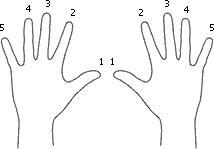
\includegraphics[scale=1]{img/fingers}
    \caption{Kairės ir dešinės rankų pirštų numeracija}
    \label{img:fingers}
\end{figure}


\section{Eksperimentinio palyginimo rezultatai}
% tablesgenerator.com - converts calculators (e.g. excel) tables to LaTeX
\begin{table}[H]\footnotesize
  \centering
  \caption{Lentelės pavyzdys}
  {\begin{tabular}{|l|c|c|} \hline
    Algoritmas & $\bar{x}$ & $\sigma^{2}$ \\
    \hline
    Algoritmas A  & 1.6335    & 0.5584       \\
    Algoritmas B  & 1.7395    & 0.5647       \\
    \hline
  \end{tabular}}
  \label{tab:table example}
\end{table}

\end{document}
